\documentclass[conference]{IEEEtran}
\IEEEoverridecommandlockouts
% The preceding line is only needed to identify funding in the first footnote. If that is unneeded, please comment it out.
%----------------------------------------------------------
\usepackage{cite}
\usepackage[pdftex]{graphicx}
% declare the path(s) where your graphic files are
\graphicspath{images/}
\DeclareGraphicsExtensions{.pdf,.jpeg,.png,.jpg}
\usepackage{amsmath,amssymb,amsfonts}
\usepackage{algorithmic}
\usepackage{graphicx}
\usepackage{textcomp}
\usepackage{array}
%\usepackage[caption=false,font=normalsize,labelfont=sf,textfon =sf]{subfig}
\usepackage{dblfloatfix}
\usepackage{url}
\usepackage{lipsum}
\usepackage{listings}
\usepackage{xcolor}
\def\BibTeX{{\rm B\kern-.05em{\sc i\kern-.025em b}\kern-.08em
    T\kern-.1667em\lower.7ex\hbox{E}\kern-.125emX}}
%----------------------------------------------------------
    \lstset{
        escapeinside={/*@}{@*/},
        language=Python,	
        basicstyle=\fontsize{8.5}{12}\selectfont,
        numbers=left,
        numbersep=2pt,    
        xleftmargin=2pt,
        frame=tb,
        columns=fullflexible,
        showstringspaces=false,
        tabsize=4,
        keepspaces=true,
        showtabs=false,
        showspaces=false,
        morekeywords={inline,public,class,private,protected,struct},
        captionpos=b,
        lineskip=-0.4em,
        aboveskip=10pt,
        extendedchars=true,
        breaklines=true,
        prebreak = \raisebox{0ex}[0ex][0ex]{\ensuremath{\hookleftarrow}},
        keywordstyle=\color[rgb]{0,0,1},
        commentstyle=\color[rgb]{0.133,0.545,0.133},
        stringstyle=\color[rgb]{0.627,0.126,0.941},
    }
%----------------------------------------------------------

\begin{document}
%\pagecolor{black}
%\color{white!100}
\title{Simulação Tinkercad\\
{\footnotesize \textsuperscript{*} Sistemas Embarcados: Prof. Marco Reis - marco.reis@ba.docente.senai.brr}

}

% \author{\IEEEauthorblockN{Marco Reis, 41650-010\IEEEauthorrefmark{1}}
% \IEEEauthorblockA{\IEEEauthorrefmark{1}Robotics & Autonomous Systems Center,
% Senai Cimatec, Salvador, Brazil}% <-this % stops an unwanted space


\author{\IEEEauthorblockN{{} João Vitor Silva Mendes}
\IEEEauthorblockA{\textit{Estudante de Engenharia Elétrica} \\
\textit{SENAI - Cimatec}\\
Camaçari, Brazil \\
joao.mendes@aln.senaicimatec.edu.br}
\and

}

\maketitle

\begin{Resumo}
  \textbf{\textit{Resumo—}Neste documento será retratado o desenvolvimento de 3 protótipos,
  utilizando o Tinkercad para desenvolver e testar o projeto
  e como microcontrolador o Arduino Uno R3. O primeiro
  protótipo a ser desenvolvido foi a calculadora, utilizando um
  teclado matricial 4x4, em que principal função é resolver
  operações matemáticas simples, porém, também foi adicionada
  a função de recursividade onde o usuário pode reutilizar o
  resultado da operação anterior. O segundo protótipo a ser
  desenvolvido foi o Dispersor de Álcool automatizado. 
  O dispersor possui um servo motor que funciona para
  abrir as portas de uma caixa, onde estava armazenado todo o
  sistema. Dentro da caixa, há um sensor de proximidade que
  irá detectar se a mão do usuário está dentro da caixa e então
  dispensar o álcool, caso não, a porta se fecharia. O último
  protótipo é um cofre, que possui um teclado matricial 4x4
  para a entrada da senha, assim o arduino pode detectar se a
  sequência está correta e então se verdadeiro abrirá a porta,
  caso seja falso manterá trancada.}

\end{Resumo}

\begin{abstract}
This document aims to describe the development of three prototypes in the class of Embebed Systems,
it was utilized the Tinkercad for design and test the project and the microcontroller used
was Arduino Uno R3. The first one is the Calculator, using a matrix keypad 4x4,
the principal function is do simple math operations, and was created a recursion function
to continue the operations. The second prototype is a Alcohol Dispenser, and the idea was a
simples system that will detect the presence of a hand and dispense alcohol.
The Dispenser have a servo motor too, to open a door for the hand, and all of the system 
will be inside a box. The last one it's a Safe Box, with a keyboard 4x4 for enter the password, 
the arduino can detect, if is correct the system can open the lock, but if the password was not correct
the system will keep locked.
\end{abstract}

\begin{IEEEkeywords}
Sistemas Embarcados, Arduino, Microcontroladores, Calculadora, Dispenser de Álcool, Cofre.
\end{IEEEkeywords}

\section{Introdução}
Durante o curso de Sistemas Embarcados, o Prof. Marco
Reis propôs o desenvolvimento de três protótipos ao longo
da primeira unidade. Desenvolvendo primeiro uma calculadora,
em seguida um dispersor de Álcool e um cofre, O sistema
utilizado para elaboração de projetos e simulações foi o
Tinkercad, ferramente gratuita pertencente a AutoDesk. Além
da utilização da plataforma de desenvolvimento Arduino Uno
R3, que foi criado originalmente para ser uma plataforma
de prototipagem open source, porém ganhou grande popular-
idade e atualmente é utilizada tanto por profissionais como
amadores.\cite{barrett2012arduino}

\section{Objetivos}
Esta atividade tem como principal objetivo aplicar as teorias computacionais desenvolvidas em sala de aula,
introduzir os alunos ao desenvolvimento de IOT's utilizando o arduino como microcontrolador, além de aprimorar
habilidades de resolução de problemas envolvendo 
sistemas embarcados.\cite{louis2016working}

\section{Componentes Utilizados}

\subsection{Calculadora}
    \begin{enumerate}
    \item Arduino Uno R3;
    \item Protoboard 400 pontos;
    \item Teclado Matricial 4x4;
    \item Resistor 200 Ω;
    \item Resistor 1 K.Ω;
    \item Fio Jumper(15u).
    \end{enumerate}
\subsection{Dispensor de Álcool}
    \begin{enumerate}
    \item Arduino Uno R3;
    \item Protoboard 800 pontos;
    \item Servo Motor 9g;
    \item Sensor Ultrassônico;
    \item Motor CC;
    \item Piezo;
    \item Push Boton;
    \item Potenciômetro;
    \item Resistor 200 Ω(3u);
    \item Capacitor 10nf;
    \item Fio jumper(12u)
    \end{enumerate}

\subsection{Cofre}
\begin{enumerate}
    \item Arduino Uno R3;
    \item Protoboard 400 pontos;
    \item Teclado Matricial 4x4;
    \item Resistor 200 Ω;
    \item Resistor 1 K.Ω;
    \item Fio Jumper(15u).
    \end{enumerate}

\section{Protótipos}
    \begin{figure}[h]
        \centering
        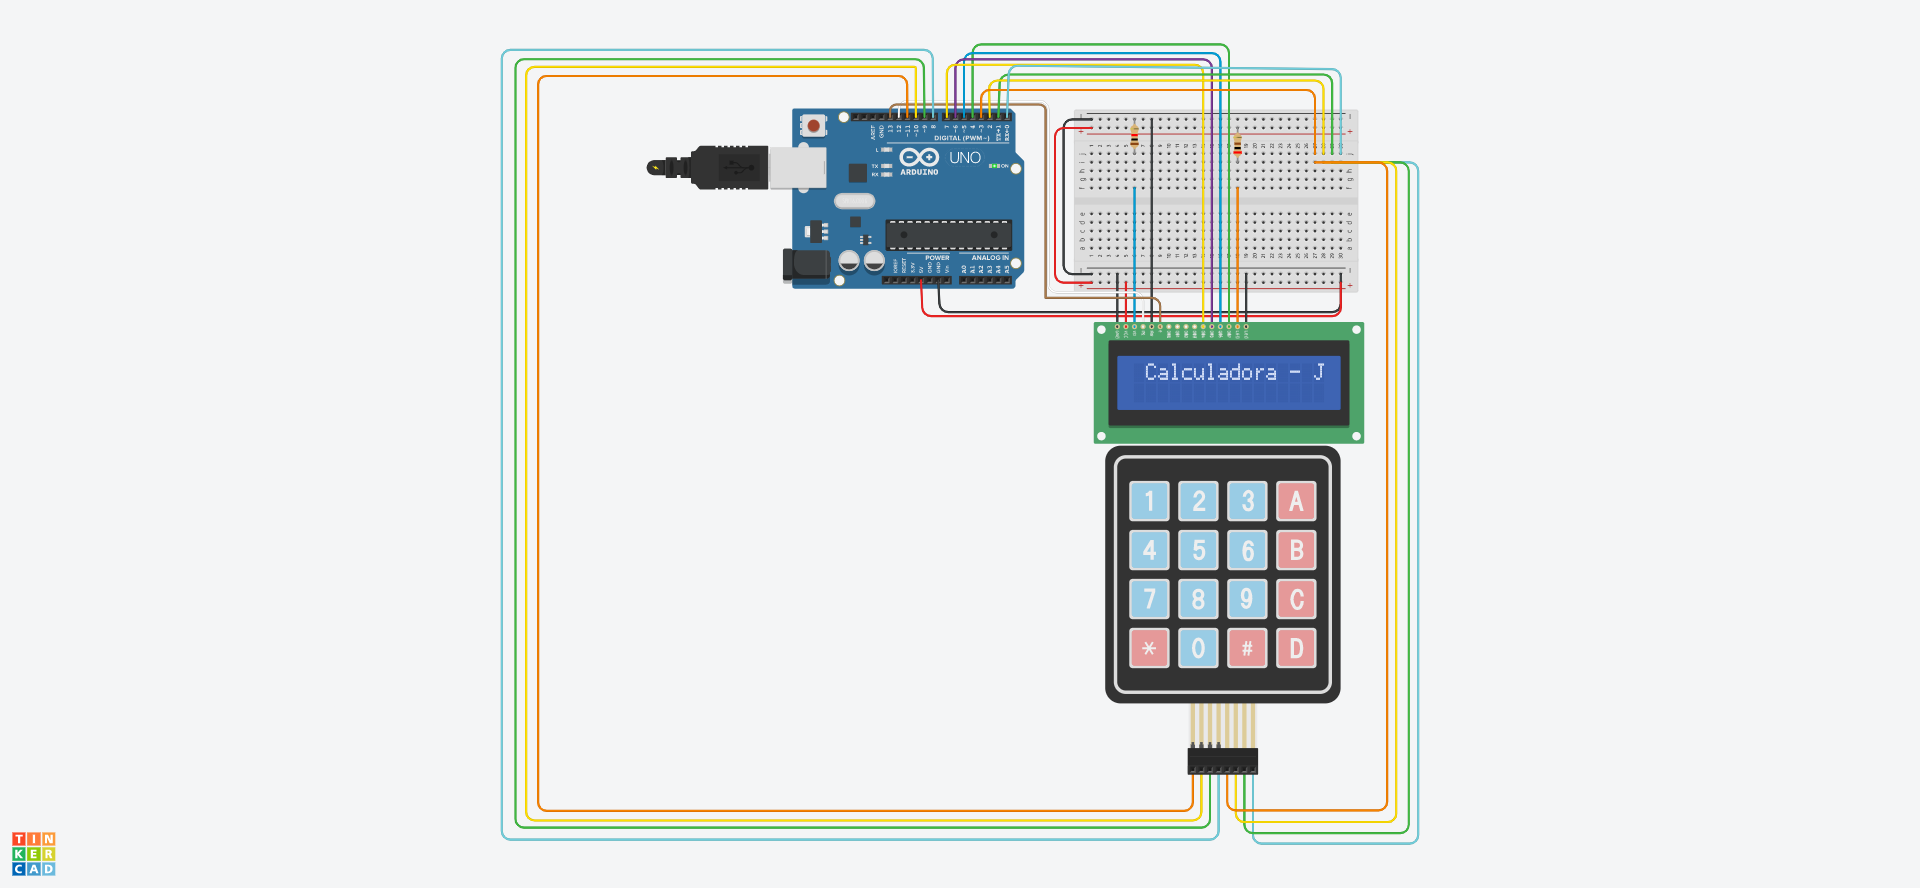
\includegraphics[scale = 0.1]{calculadora.png}
        \caption{Protótipo Calculadora.}
        \label{Calculadora}
    \end{figure}

    \begin{figure}[h]
        \centering
        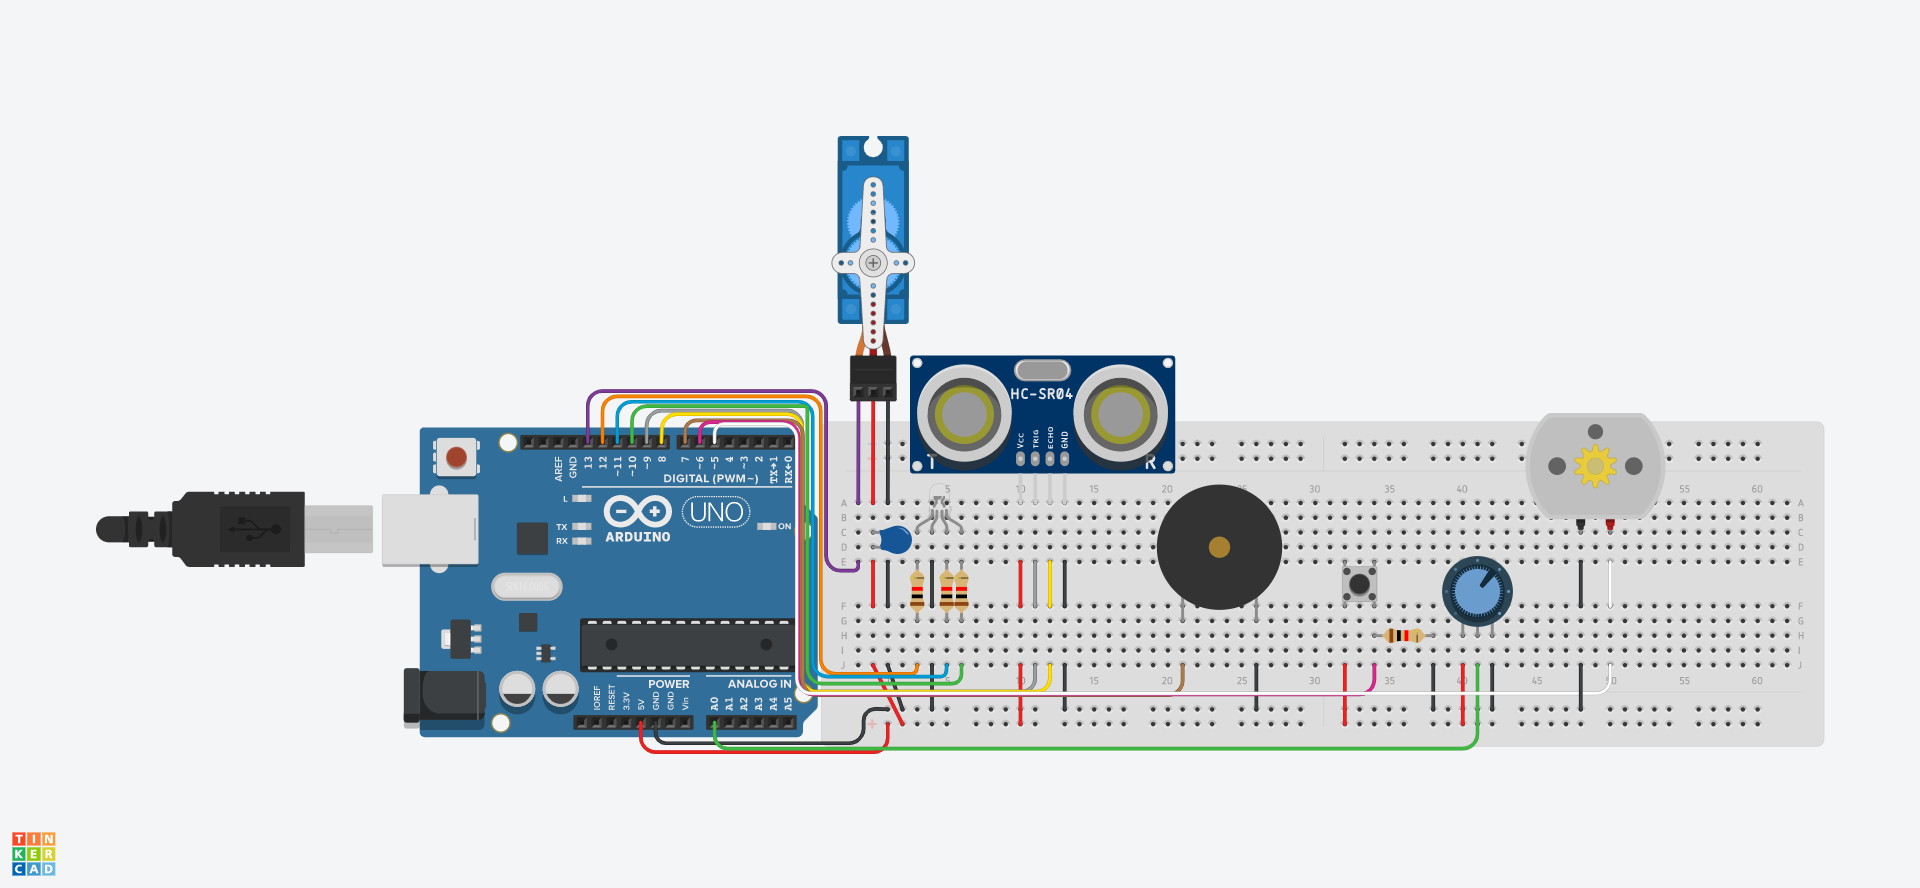
\includegraphics[scale = 0.1]{dispenser.png}
        \caption{Protótipo Dispensor de Álcool.}
        \label{Calculadora}
    \end{figure}

    \begin{figure}[h]
        \centering
        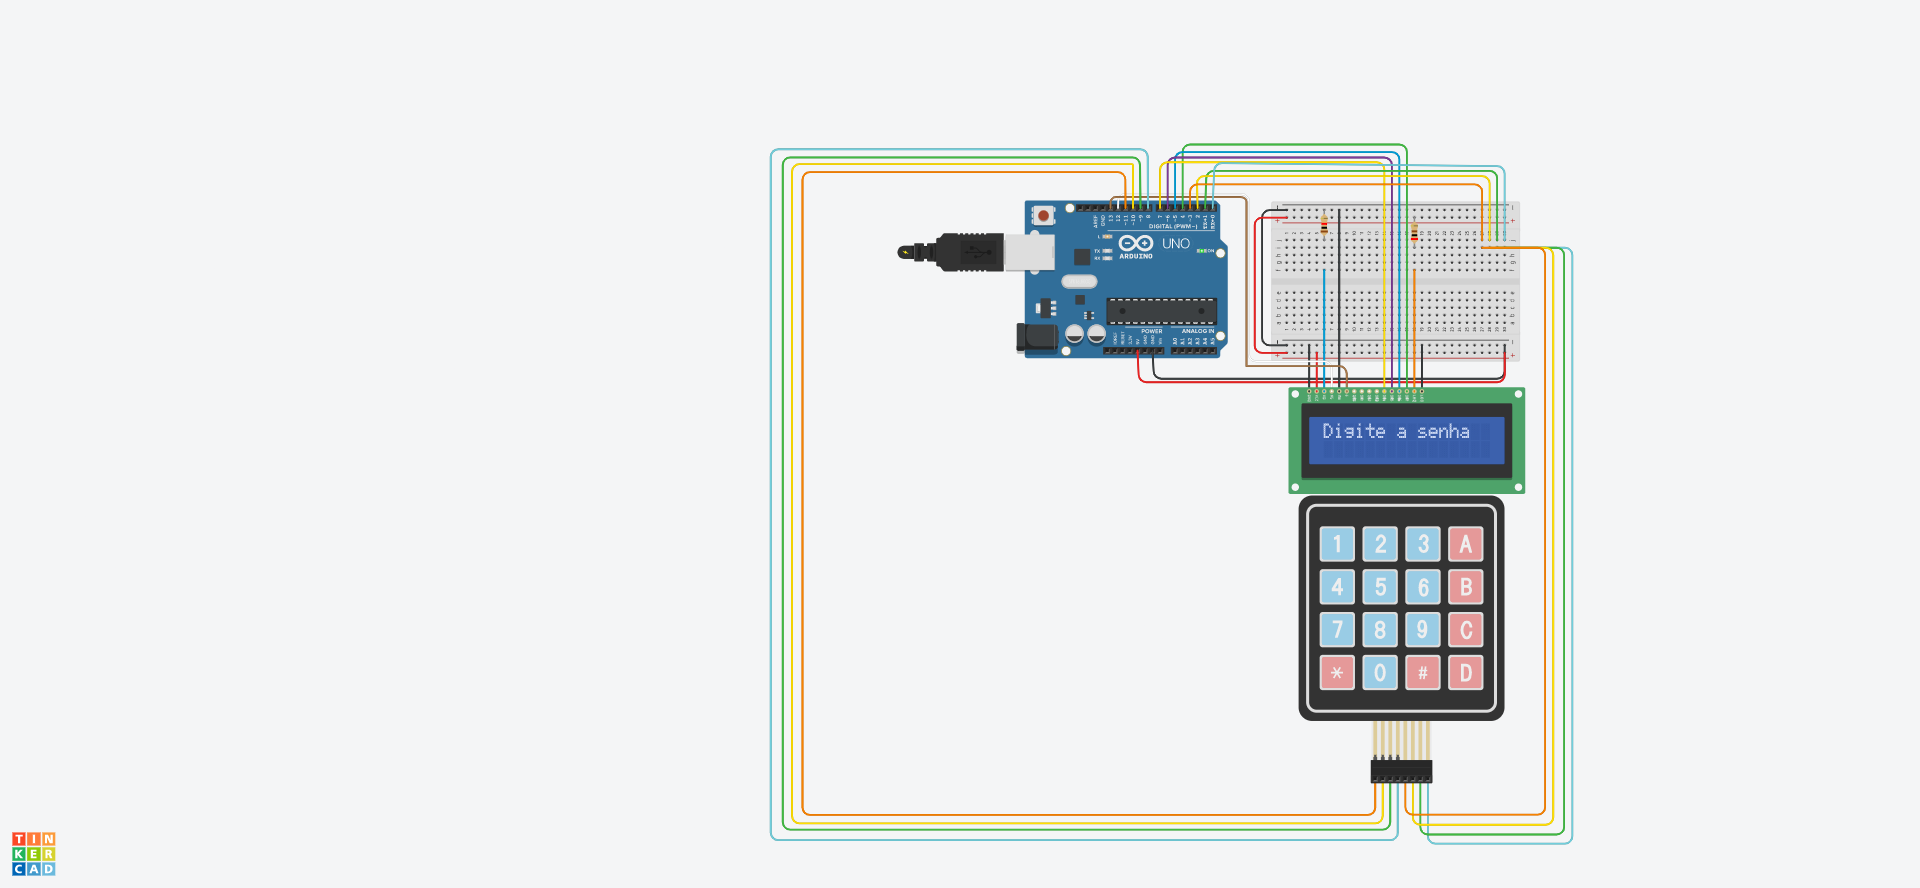
\includegraphics[scale = 0.1]{cofre.png}
        \caption{Protótipo Cofre.}
        \label{Calculadora}
    \end{figure}

\section{Códigos}
    \subsection{Calculadora}
        \begin{lstlisting}  
    #include <Keypad.h>
    #include <Wire.h>
    #include <LiquidCrystal.h>
    #include <stdio.h>
        \end{lstlisting}
        Aqui é possível analisar quais bibliotecas foram utilizadas para o desenvolvimento da calculadora. 
        A Keypad.h é utilizada para ter acesso as funções do teclado
        matricial, assim como a LiquidCrystal.h para obter acesso ao
        pacote de funções para controlar a tela LCD. A biblioteca
        Wire.h tem como função garantir a interação entre o Arduino
        e os dispositivos conectados, já a biblioteca stdio.h foi utilizada
        para dar acesso as funções mais básicas da linguagem C++.
        \begin{lstlisting}  
    char customKey, start;
    const byte ROWS = 4;
    const byte COLS = 4;
    char keys[ROWS][COLS] = {
        {'1','2','3','+'},
        {'4','5','6','-'},
        {'7','8','9','*'},
        {'C','0','=','/'}
        };
    byte rowPins[ROWS] = {11,10,9,8};
    byte colPins[COLS] = {3,2,1,0};
    Keypad customKeypad = Keypad(makeKeymap(keys), rowPins, colPins, ROWS, COLS);
    \end{lstlisting}
          A declaração das variáveis do teclado matricial é feita da
      seguinte forma. Primeiro há a definição das variáveis que
      serão utilizadas, depois é construı́da uma matriz key do tipo
      char que será orientada pelas variáveis ’ROWS’ e ’COLS’,
      respectivamente linhas e colunas. Além disso é definido na
      linha 13 os pinos do teclado, baseando-se nas declarações
      feitas anteriormente na linha 11 e 12 que define os pinos em
      relação a matriz declarada na linha 4.

        \begin{lstlisting} 
    const int rs = 12, en = 13, d4 = 7, d5 = 6, d6 = 5, d7 = 4;
    LiquidCrystal lcd(rs, en, d4, d5, d6, d7);
        \end{lstlisting}
        Neste bloco de código é definido as variáveis que representaram os pinos da tela lcd 16x2.
        Na linha 2 essas variáveis são definidas para cada porta do LCD.

        \begin{lstlisting}
    double first = 0;
    double second = 0;
    double third = 0;
    double total = 0;
        \end{lstlisting}
        Neste bloco são definidas as variáveis do tipo double que representaram
        os números a serem cálculados durante o loop.

        \begin{lstlisting}
void setup(){
  lcd.begin(16, 2);
  for(int i=0;i<=20;i++){
    lcd.setCursor(5,0);
    lcd.print("Calculadora - Joao Vitor");
    delay(100);
    lcd.scrollDisplayLeft();
    delay(100);
  	}
  lcd.clear();
  lcd.setCursor(0,0);		
			  }
        \end{lstlisting}
        Na função setup é inicializado o LCD, após isso um loop
        que apresenta o título do protótipo e em seguida a função
        lcd.scrollDisplayLeft() para os caracteres mudarem de posição
        e apresentar toda a frase.
        
        \begin{lstlisting}
void loop(){
    customKey = customKeypad.getKey();
    switch(customKey){
        case '0'...'9':
        lcd.setCursor(0,0);
        first = first * 10 + (customKey - '0');
        lcd.print(first);
        break;
    
        case '+':
            if(first != 0){
                lcd.setCursor(15,1);
                lcd.print("+");
                second = SecondNumber();
                total = first + second;
                lcd.setCursor(0,3);
                lcd.print(total);
                first = 0;
                second = 0;
                }
                else if(first == 0){
                third = ThirdNumber(total, '+');
                total = total + third;
                lcd.setCursor(0,3);
                lcd.print(total);
                third = 0;
                }
        break;

        case 'C':
        total = 0;
        first = 0, second = 0;
        lcd.clear();
        break;
        }
    }
        \end{lstlisting}

        Na função loop será o local em que os cálculos serão
        efetuados. No primeiro momento é utilizada a função getkey()
        associada a variável definida para representar o teclado é
        possível obter o que o usuário está digitando, e o retorno dessa
        função que será um char é empregado a variável 'customKey'.
        Logo após isso, o código segue para um switch onde é possível
        entrar em 6 alternativas, a primeira que representa os números
        de 0 a 9, a segunda até a quinta que representarão as operações
        caso o usuário dê a entrada no teclado(no código acima é
        representado apenas o caso da operação soma, com intuito de
        simplificar o processo já que os casos das demais operações
        funcionam da mesma forma), e por último o caso ’C’.
        No caso ’0...9’ representado na linha 3, tem como função
        formar o primeiro número que será alocado na variável ’first’.
        Porém, na primeira tentativa de execução o código na linha
        6, possuía o seguinte formato: (first = first + customKey),
        e com isso apresentava na tela o código ASCII, designado
        para cada carácter que representava um número. Para corrigir
        este problema o customKey passou a subtrair o código ASCII
        que representava o carácter ’0’, para possuir o seu real valor.
        Para a variável first poder receber mais de um algorismo foi
        necessário incrementá-la de forma que o seu próprio valor
        fosse multiplicado por uma dezena e assim somado ao novo
        valor recebido pela variável ’customKey’ subtraindo o valor
        em ASCII do carácter ’0’. Após cada digito o código executa
        a função lcd.print() que imprimirá na tela do usuário cada
        algorismo digitado.
        Quando o usuário termina de digitar o primeiro número é
        esperado a entrada de uma das 4 operações, nesse exemplo
        será utilizada a operação da soma. Quando houver a entrada
        da operação soma, o código entrará no case ’+’ iniciado na
        linha 10, o programa primeiro verifica através de uma estrutura
        de decisão se o usuário já deu a entrada do primeiro número,
        se sim o usuário prosseguirá com o laço, caso não o usuário
        voltará ao inicio do loop, obrigando o usuário a dar a entrada
        de um valor. Porém, se já houver esse primeiro número. o
        código entrará na estrutura if e seguirá o seguinte processo:
        é impresso na tela nas coordenadas (15,1) como mostra a
        função lcd.Setcursor() a operação a ser executada. Após isso é
        utilizada a função SecondNumber(), o código da função segue
        abaixo.\cite{table2007ascii}
        \begin{lstlisting}
            long SecondNumber(){
  while( 1 ){
    customKey = customKeypad.getKey();
    if(customKey >= '0' && customKey <= '9'){
        second = second * 10 + (customKey - '0');
        lcd.setCursor(0,1);
        lcd.print(second);
        }

    if(customKey == '=') break;
            } 
  return second;
					}
        \end{lstlisting}
        
        A função SecondNumber segue uma lógica parecida com a
        utilizada no case ’0...9’, mas no lugar de uma função loop é
        utilizada um laço de repetição while. Além disso, é utilizado
        outra estrutura if com intuito de verificar se algum momento
        será pressionada a tecla que representa o sinal ’=’ que iria
        interromper o loop. Com o fim da função ela retornará uma
        variável do tipo long. De volta a função loop, na linha 14
        a variável ’second’ recebe o valor retornado para a função,
        que em segui é somado com o valor de ’first’ e atribuído a
        variável ’total’, assim o valor é imprimido na segunda linha
        da tela com o sinal de ’=’. Ao final, os valores de ’first’ e
        ’second’ são zerados
        O programa repetirá esse mesmo processo até ser encerrado
        se seguir essa mesma lógica de entrada. Porém, a função
        ThirdNumber() foi adicionada com intuito de poder usar o
        valor totalizado pela operação anterior em uma nova operação,
        tornando a calculadora recursiva. Desse modo, se analisarmos 
        o caso em que o usuário entra com o valor de uma
        operação mesmo com as variáveis ’first’ e ’second’ zeradas,
        é possível fazer a operação entre o terceiro número digitado
        pelo usuário com o valor totalizado anteriormente. A função
        ThirdNumber() é localizada na estrutura Else If, nos casos de
        operação dentro do switch, estes que verificam se é possível
        fazer a recursão explicada anteriormente. 
    \begin{lstlisting}
long ThirdNumber(double r, char op){
  lcd. clear();
  lcd.setCursor(0,0);
  lcd.print(r);
  lcd.setCursor(15,1);
  lcd.print(op);
  while( 1 ){
    customKey = customKeypad.getKey();
    if(customKey >= '0' && customKey <= '9'){
        third = third * 10 + (customKey - '0');
        lcd.setCursor(0,1);
        lcd.print(third);
        }
        
    if(customKey == '=') break;
        }
  return third;
					}
    \end{lstlisting}

    Esta função segue a mesma lógica que a função Second-
    Number(), porém antes de entrar no laço de repetição, o
    programa faz algumas alterações visuais na tela para imprimir
    o valor da variável ’total’ representado agora pela variável ’r’
    e é impresso também a operação atribuída a variável ’op’, estas
    variáveis são recebidas pela função ainda na linha 21 da função
    loop(). Por fim, é retornado um valor long
    que será recebido pela variável ’third’. O processo segue o
    mesmo padrão na função loop() das demais operações feitas
    anteriormente.
    
    \subsection{Dispensor de Álcool}
    No código para o dispersor de álcool a única biblioteca
    utilizada é a Servo.h, que permite o acesso a funções para o
    funcionamento do servo motor.
    \begin{lstlisting}
//HEADERS
#include <Servo.h>
// SETSENSOR
    byte pinoTransmissor = 9; // trig
    byte pinoReceptor = 8; // echo
	float cm ,duracao; // comprimento de onda/ tempo de resposta
//SET LED RGB
	const byte R = 12;
	const byte B = 11;
  	const byte G = 10;
//SET PUSH BOTON
  const int botao = 6; 
  int estadoBotao = 0;
//SET SERVO MOTOR
	int pinServo = 13;
	Servo s;
	int angulo = 0;
//MOTOR
  int pin_motor = 5;
  float motor;
        \end{lstlisting}
        Neste trecho de código é possível analisar as declarações de
        variáveis utilizadas e também dos dispositivos utilizados no
        sistema. A partir do comentário ”SETSENSOR”, é declarado
        para o sistema os pinos que são ligados ao sensor, no caso das
        portas trig e echo, além das variáveis ’cm’ e 'duracao', 
        que irão obter os valores de distância e tempo em que a sonda irá até o objeto e voltará.
        Em seguida é declarada as variáveis referentes
        ao LED RGB que está presente no sistema para representar a
        distância da mão do usuário até o sensor. A partir do cometário
        ”SETPUSHBOTON” é declarada as variáveis que representam
        o pino do botão e o estado do botão, respectivamente as
        variáveis ’botão’ e ’estadoBotao’. A partir de ”SETSERVO” é
        definida as variáveis do servo motor, primeiro é definido o pino
        do servo motor, em seguida uma variável ’s’ que representará
        o motor durante todo o código e um inteiro que armazenará o
        angulo de rotação. Por último, é definido o pino do motor é
        definido e uma variável ’motor’ para receber do potenciômetro
        a velocidade em que o motor irá descarregar o álcool.
        \begin{lstlisting}
void setup(){
    // LED and PUSH BOTON
    pinMode(R, OUTPUT);
    pinMode(G, OUTPUT);
    pinMode(B, OUTPUT);
    // sensor
    pinMode(pinoTransmissor, OUTPUT); // transmissor
    pinMode(pinoReceptor, INPUT);     // receptor
    //porta serial
    Serial.begin(9600);
    //servo
    s.attach(pinServo);
  	s.write(0);
  	//boton
 }
        \end{lstlisting}

        Na função setup em primeiro momento associa os pinos
        do LED RGB a saı́da de dados, logo após é definido o pino
        transmissor como saı́da de dados e o pino receptor como
        entrada de dados. Com isso, é iniciado o serial e definida
        a variável associada ao pino do servo motor para o
        sistema e executando a função servo.write() associada a variável 's' que representa o servo motor na posição '0', para
        indicar a posição em que o servo deve iniciar. Para entender
        a função loop é necessário antes entender algumas funções
        que serão utilizadas. As primeiras a serem retradas serão as
        funções deseginadas a orientar o funcionamento do LED RGB.

        \begin{lstlisting}
 void red(){
    analogWrite(R, 255);
    analogWrite(G, 0);
    analogWrite(B, 0);
  }
void green(){
    analogWrite(R, 0);
    analogWrite(G, 255);
    analogWrite(B, 0);
  }  
void blue(){
    analogWrite(R, 0);
    analogWrite(G, 0);
    analogWrite(B, 255);
  }  
void apaga(){
    analogWrite(R, 0);
    analogWrite(G, 0);
    analogWrite(B, 0);
  } 
        \end{lstlisting}
        As funções red(), green() e blue() são chamadas com intuito de acionar o LED com 3 cores diferentes que representarão a distância entre a mão do usuário e o sensor.
        E no caso da função apaga(), é utilizada para apagar o led quando o funcionamento do sensor for interrompido.
        \begin{lstlisting}
void gira(){
    angulo = 250;
    s.write(angulo); 
    delay(1000);
   
 	}

void volta(){
    angulo = 0;
    s.write(angulo); 
    delay(1000);
 	}
        \end{lstlisting}
        As funções gira() e volta() são utilizadas para orientar o
        funcionamento do servo motor, que será responsável por abrir e fechar a porta do sistema de higienização, após o giro do
        servo motor, há também no código uma função delay() para o
        sistema de higienização funcionar apenas quando o dispositivo
        abrir ou fechar a porta por completo.

                \begin{lstlisting}
float distancia(){  
  
  digitalWrite(pinoTransmissor, LOW);
  delayMicroseconds(5);
  digitalWrite(pinoTransmissor, HIGH); 
  delayMicroseconds(10);
  digitalWrite(pinoTransmissor, LOW);
  duracao = pulseIn(pinoReceptor, HIGH);
  float calcDistancia= (duracao/2) * 0.0343; 
  
  return calcDistancia;  
    }
        \end{lstlisting}
        A última função a ser criada é a distancia(), que serve
        para fazer o cálculo da distância da mão do usuário até
        o sensor ultrassônico. Em primeiro momento são enviados
        pulsos através da função digitalWrite(), dois baixos e um alto,
        sendo eles intercalados, com intervalo de 5 microssegundos do
        primeiro para o segundo, e 10 microssegundos do segundo para
        o terceiro. Após isso, é chamada a função pulseIn() que recebe
        o tempo em que o pulso levou para ir até o objeto e voltar,
        este dado é armazenado na variável ’duracao’. O próximo
        passo é definida uma variável float, chamada ’calcDistancia’
        que receberá o resultado de um cálculo envolvendo o produto
        entre a velocidade do som(em centímetro por microssegundos)
        e a metade do tempo em que o pulso levou para ir ao
        objeto e voltar. Por fim, é retornado o valor da distância em
        centímetros.


        \begin{lstlisting}
void dispense(){
    motor = analogRead(A0)/4;
    analogWrite (pin_motor, motor);
    delay(2000);
    analogWrite(pin_motor, 0);
    tone(7, 100, 200);
    while(cm<50){
        cm = distancia();
        if(cm>50){ 
          green();
          delay(1000); 
          volta();
          }
    	}
	}
        \end{lstlisting}
        A função dispense() orienta o sistema a dispensar o álcool
        e como dispensar. Em primeiro momento a variável motor
        irá receber informações da porta analógica ’A0’, que está
        conectada a um potenciômetro de 10K.ohm, dessa forma
        regulando a velocidade do motor, consequentemente a quantidade 
        de liquido a ser dispersado. Logo após, a função
        analogWrite() recebe duas informações, primeiro o pino do
        motor e a variável ’motor’ que recebeu o valor da intensidade
        da corrente a ser enviada para o motor CC. Durante a dispersão
        o código apresenta uma função delay() que irá regular também
        a quantidade de álcool a ser expelido pelo tempo de dispersão(Definido por padrão pelo sistema 1000ms),
        após esse intervalo de tempo, uma outra função analogRead()
        irá receber as informações para interromper o funcionamento
        do motor CC. Por fim, um Piezzo localizado na porta 7, é
        acionado pela função analogWrite(), a fim de avisar ao usuário
        que a dispersão já foi realizada. Durante a primeira fase de
        desenvolvimento, o código da função dispense() acabava nesse
        momento, após sair da função, havia outra função volta()
        que fecharia a porta do sistema, porém, neste caso o sistema
        poderia fechar a porta com a mão do usuário ainda dentro do recipiente. 
        A segunda solução foi colocar um delay, mas ainda não era algo eficiente.
        Contudo, como o sistema possui um sensor para verificar
        a distância, o código passou a conter um laço de repetição 
        que se repetiria até o momento que o sensor não verificasse mais a mão
        do usuário dentro do sistema, com isso permitindo que o
        mecanismo fechasse a porta do sistema.
        \begin{lstlisting}
void loop(){
  estadoBotao = digitalRead(botao);          

  if (estadoBotao == HIGH){
    gira();
    blue();
    cm =  distancia();
    if(cm >0 && cm<=30){ 
      red(); 
      dispense(); 
    else if (cm >50 && cm<=100) {
        green();
        volta();

    }
    else if (cm>100) {
        blue();
        volta();

    }
    else {
        volta();
        apaga();
    }   
 
  }
        \end{lstlisting}
        Enfim, na função loop(), em primeiro momento é checado
        o estado do botão e armazenado na variável ’estadoBotao’,
        após a verificação se o botão estiver apertado ele entre em
        uma estrutura if, caso não ele segue repetindo o loop. Ao
        entrar na estrutura, a função gira() é acionada e a porta abre
        e acende o led azul para indicar que o usuário pode colocar
        a mão. Após isso a variável ’cm’ recebe a distância da mão
        do usuário da função distancia(), com isso uma estrutura de
        seleção verifica a distância e responde através do LED RGB,
        azul para vazio, verde para indicar que a mão do usuário ainda
        está muito longe e vermelho para indicar que a distância está
        correta e só então é dispensado o fluido através da função
        dispense(). Vale lembrar que dentro da função dispense existe
        um mecanismo para verificar se o usuário já tirou a mão e só
        então o mecanismo fecha a porta do sistema.

    \subsection{Cofre}
        \begin{lstlisting}
#include <Keypad.h>
#include <Wire.h>
#include <LiquidCrystal.h>
#include <stdio.h>
#include <string.h>
        \end{lstlisting}
        Até a linha 4 as bibliotecas inclusas já foram discutidas
        neste relatório, porém, neste projeto de cofre há a adição
        de uma nova biblioteca, chamada de string.h com intuito
        de acessar funções para manipular strings. Em suma, outras
        declarações também já foram expostas neste relatório e não
        serão abordadas novamente, como a declaração do teclado
        matricial e do display 16x2. Sendo assim, o próximo ítem a
        ser abordado será a função setup() e declaração das variáveis
        utilizadas durante o programa.
        \begin{lstlisting}
char pass[3];
int cmp, cont, tentativas, chave = 1;

Keypad customKeypad = Keypad(makeKeymap(keys), rowPins, colPins, ROWS, COLS);

void setup(){
  
  lcd.begin(16, 2);
  strcpy(pass, "0000");
  tentativas = 0;
  
}
        \end{lstlisting}
        Na linha 1 é declarada a variável ’pass’ do tipo string que terá
        4 caracteres, esta armazenará a entrada do usuário. Logo, após
        há a declaração dos inteiros, primeiro ’cmp’ que receberá o
        retorno da comparação entre a senha do sistema e a entrada do
        usuário. A variável ’cont’ funcionará como um contador dentro
        do loop(), tentativas irá verificar quantas vezes o usuário errou
        a senha e se exceder o limite destruirá os dados do cofre. Por
        fim, a chave que irá auxiliar a interrupção do funcionamento
        do cofre caso o usuário exceda o limite de erros. Na função
        setup(), é iniciado o LCD, após isso é atribuído a variável
        ’pass’ a string ’0000’, as tentativas são zeradas.
        \begin{lstlisting}
void correct(){
  lcd.clear();
  strcpy(pass, "0000");
  cont = 0;
  lcd.setCursor(0,0);
  lcd.print("Destrancado");
  delay(2000);
  tentativas = 0;
}
        \end{lstlisting}
        A função correct() será responsável por enviar para o usuário
        a mensagem que o cofre está destrancado e zerar as variáveis
        que serão utilizadas novamente.        
        \begin{lstlisting}
void incorrect(){
  lcd.clear();
  strcpy(pass, "0000");
  cont = 0;
  lcd.setCursor(0,0);
  lcd.print("SENHA NEGADA!");
  delay(2000);
  lcd.clear();
  if(tentativas == 3) autodestruir();
}
        \end{lstlisting}
        A função incorrect() funciona da mesma forma que a função correct(), porém envia o sinal que a senha ta negada. Porém, se o número de tentativas for excedido, a função autodestruir() é acionada.
        \begin{lstlisting}
void autodestruir(){
  int i;
 for(i = 3; i >= 0; i--){ 
 lcd.clear();
 lcd.setCursor(0,0);
 lcd.print("Destruicao");
 lcd.setCursor(0,1);
 lcd.print("arquivos em: ");
 	lcd.print(i);
   	delay(1000);
 }
  chave = 0;
}
        \end{lstlisting}
        A função autodestruir() em primeiro momento declara um
        inteiro ’i’ que será o contador da estrutura de repetição for a
        seguir. Esta estrutura servirá para iniciar a contagem regressiva
        e imprimir na tela para o usuário, avisando que os dados
        serão destruídos, apagando e imprimindo novamente a mesma
        mensagem, mudando apenas o valor do inteiro ’i’. Após isso
        a chave é zerada e o programa irá parar de funcionar.
        \begin{lstlisting}
void verifica(){
  cmp = strcmp("2507", pass);
  lcd.setCursor(5,0);
  if(cmp == 0) correct();
  else incorrect();
  tentativas++;
}
        \end{lstlisting}
        A função verifica() tem como objetivo verificar se a entrada do usuário é igual a senha determinada pelo sistema, através da função strcmp.
        A variável 'cmp' recebe o retorno da comparação que se for positivo é igual a '0'. Logo após, uma estrutura de if analise se 'cmp' for igual a '0',
        é acionada a função correct(), senão é acionada a função incorrect() e o número de tentativas é incrementado o valor de uma unidade.

        \begin{lstlisting}
void loop(){

  while(chave == 1){
      lcd.setCursor(0,0);
      lcd.print("Digite a senha");
      customKey = customKeypad.getKey();

      switch(customKey){

          case '0'...'9':
            lcd.setCursor(0,1);
            if(cont < 4){
              pass[cont] = customKey;
              lcd.print(pass);
              cont++;		}
              else{
              verifica();	}

              break;

          case 'C':
              lcd.clear();
              strcpy(pass, "0000");
              cont = 0;
              break;

          case '#':
              verifica();
              break;


              }
  } if(chave == 0){
    lcd.clear();
    lcd.setCursor(0,0);
    lcd.print("ERROR");
  	}

  }
        \end{lstlisting}
        Na função loop(), é iniciado um laço de repetição while,
        para enquanto a chave for igual a ’0’ o programa continuará
        funcionando, caso não o programa irá parar de funcionar.
        Então, é impresso na tela LCD para o usuário a mensagem
        ’Digite a senha’, com isso a variável ’customKey’ receberá
        a entrada do usuário de um carácter. Com isso entra em
        um switch baseado na variável ’customKey’, se a entrada do
        usuário for um número, entrará no case ’0...9’, a estrutura if
        irá verificar se o ’cont’ está abaixo de quatro, que é o número
        máximo de caracteres por senha, com isso a variável ’pass’
        irá receber esses caracteres que o usuário digitar no teclado,
        assim que atingir o usuário der entrada de ’’ para verificar a
        senha ou exceder o número limites de dígitos o programa irá
        entrar na função verifica(). Como dito antes, no caso da entrada
        ’’, a função verifica() será chamada, ou no caso da entrada
        ser igual a ’C’ será zerado tanto a variável ’pass’ quanto a
        variável ’cont’ e a tela LCD será limpada. Caso a função
        autodestruir() seja chamada, o laço while será interrompido,
        e então é impresso no LCD a mensagem de ”ERROR” e o
        programa sera quebrado.
\section{Conclusão}
Baseado-se nas simulações realizadas no TinkerCAD, os
experimentos concluíram todos os objetivos propostos com
sucesso. A elaboração dos protótipos permitiu a aplicação
da teoria computacional desenvolvida em sala de aula, além
de desenvolver outras habilidades essenciais para desenvolvimento 
de IOT’s, como as aplicações da Lei de Ohm,
elaboração de circuitos elétricos simples e programação de
sistemas embarcados.


    \bibliographystyle{IEEEtran}
    \bibliography{Bibliography}
    
    


\end{document}